\documentclass[11pt]{article}

\usepackage{fullpage}% reasonable margins
\usepackage{array} % makes tables nicer
\usepackage{multirow} %tables
\usepackage{comment} %block comments
\usepackage{color} %colored text
\usepackage{graphicx} %images
\usepackage{enumerate}
\usepackage{enumitem} 

%squeezed itemize for table.
\newenvironment{packed_itemize}{
\begin{itemize}
  \setlength{\itemsep}{1pt}
  \setlength{\parskip}{0pt}
  \setlength{\parsep}{0pt}
}{\end{itemize}}

\title{\bf YAExS Stakeholder Review 1}
\author{TimeFinders: Andrew Karnani, Auston Sterling, Jeffrey Rodowicz, Vera Axelrod}
\date{October 29, 2012}

\begin{document}
\maketitle

%%%%%%%%%%%%%%%%%%%%%%%%%%
%%%%%%%%%%%%%%%%%%%%%%%%%%
\section*{Demonstration} % ANDREW + AUSTON %
%%%%%%%%%%%%%%%%%%%%%%%%%%
\textcolor{red}{
The team must present a demo that shows the feature implementation of the list of features promised during Elaboration from their schedule.
Vera: I'm not sure if we need to write anything for this.}



%%%%%%%%%%%%%%%%%%%%%%%%%%
%%%%%%%%%%%%%%%%%%%%%%%%%%
\section*{Sequence Diagrams} % VERA %
%%%%%%%%%%%%%%%%%%%%%%%%%%
\begin{comment}
\textcolor{red}{
Interaction diagrams showing how a specific Use Case is realized within the beta version of the software. The diagrams must use correct UML notation.  Check for proper UML, and makes sense.}
\end{comment}

A sequence diagram for the log-in use case is shown in figure \ref{fig:logInSeq}
 while figure \ref{fig:startSeq} shows a sequence diagram for the start scheduling 
use case.  We have also included a sequence diagram for the ``could" implement feature view schedule, shown in figure \ref{fig:viewSeq}. 

\begin{figure}
	\centering
		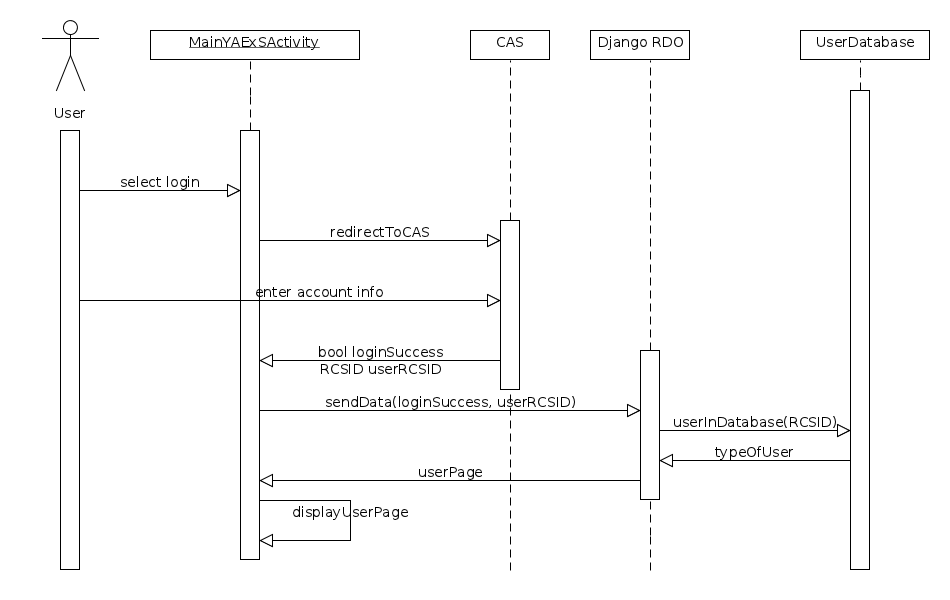
\includegraphics[width = \textwidth]{logInSequence.png}
	\caption{Log-In Sequence Diagram}
	\label{fig:logInSeq}
\end{figure}

\begin{figure}
	\centering
		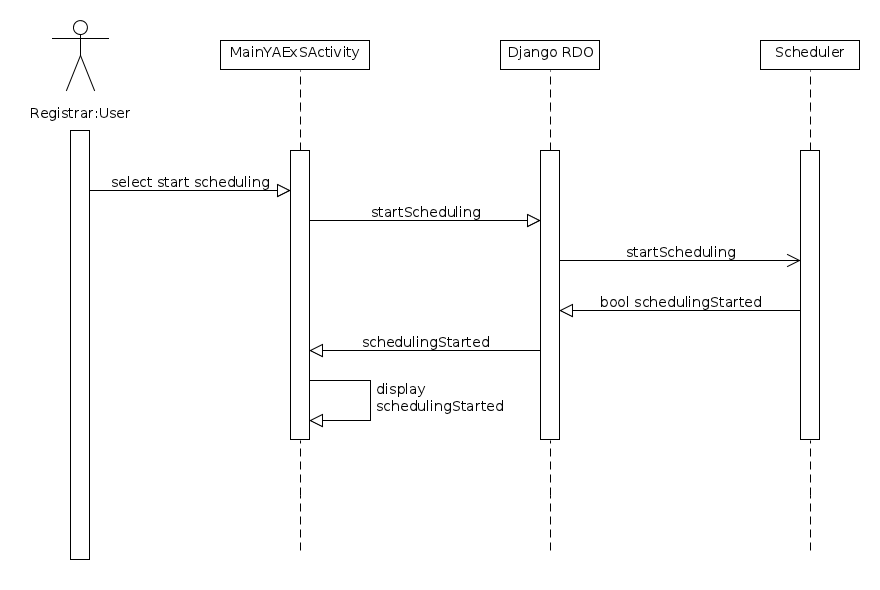
\includegraphics[width = \textwidth]{startSchedulingSequence.png}
	\caption{Start Scheduling Sequence Diagram}
	\label{fig:startSeq}
\end{figure}


\begin{figure}
	\centering
		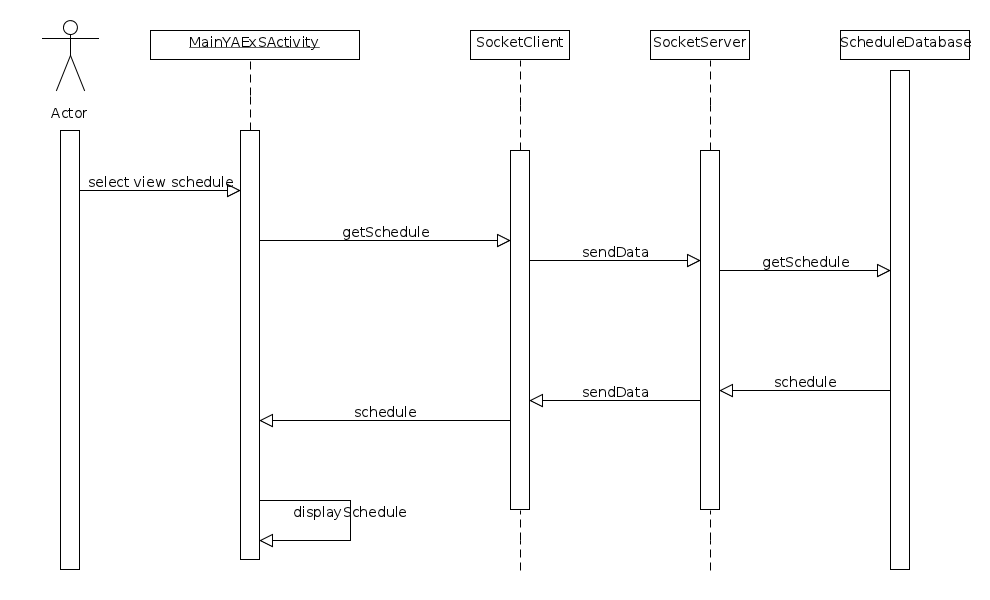
\includegraphics[width = \textwidth]{viewScheduleSequence.png}
	\caption{View Schedule Sequence Diagram}
	\label{fig:viewSeq}
\end{figure}



%%%%%%%%%%%%%%%%%%%%%%%%%%
%%%%%%%%%%%%%%%%%%%%%%%%%%
\section*{Static Class Diagrams}  % VERA %
%%%%%%%%%%%%%%%%%%%%%%%%%%
\textcolor{red}{
A static class diagram of the project's internal software structure. The diagram must be valid UML and accurately depict the software.  Check for proper UML, and makes sense.}



\begin{figure}
	\centering
%		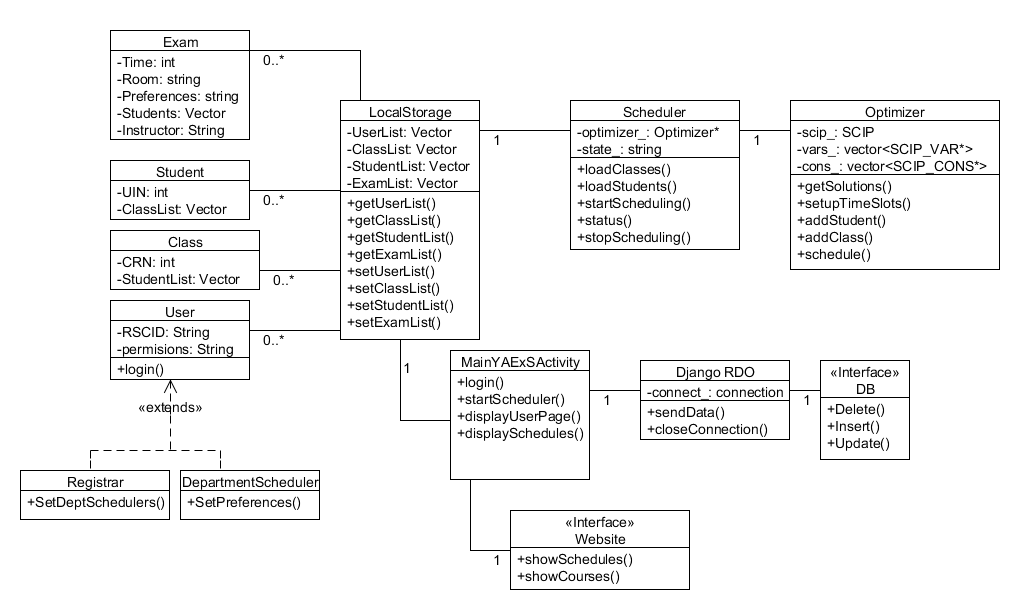
\includegraphics[width = \textwidth]{staticClassDiagram.png}
	\caption{Static Class Diagram}
	\label{fig:staticDiagram}
\end{figure}


%%%%%%%%%%%%%%%%%%%%%%%%%%
%%%%%%%%%%%%%%%%%%%%%%%%%%
\section*{ Design Approach}  % JEFF? %
%%%%%%%%%%%%%%%%%%%%%%%%%%
\textcolor{red}{
Submit your design approach (**must be object-oriented) and any design patterns you plan on using in your code. Approach should be clearly articulated and mention at least one design pattern.}

Our team broke our project into two main sections, our website, including our database, and the scheduler itself. The main design pattern that we are implementing will be the Model–view–controller pattern. Our model being the database and the final exam schedule that will be produced, the view being what the website shows to the end user, and the controller being the user interface of the website and the scheduling program. We have created a framework for communication between the scheduling program and SCIP, our schedule solver. We have created a Postgres database that will be storing all of our data centrally, and are working on creating a standard for the data that will be contained, which depends on the data that we are able to obtain from the registrar. Both our website and our scheduling program are being designed in a modular way, which will enable us to implement one case at a time and is conducive to the iterative approach that we are taking.


%%%%%%%%%%%%%%%%%%%%%%%%%%
%%%%%%%%%%%%%%%%%%%%%%%%%%
\section{Contribution Summary} % ALL %
%%%%%%%%%%%%%%%%%%%%%%%%%%
\begin{tabular}{|m{1.4in}|m{4in}|}
\hline 
\textbf{\large Name}     & \textbf{\large Contributions} \\
\hline\hline

 Andrew Karnani
	&
	 \begin{packed_itemize}
		\item Created Database Skeleton
		\item Designed Website User Interface Prototypes
		\item Tested CAS Authentication
	\end{packed_itemize}
\\
\hline
 Auston Sterling
	&
	 \begin{packed_itemize}
	        \item Created Scheduler Code Skeleton
		  \item Set Up SCIP
	\end{packed_itemize}
\\
\hline
Jeffrey Rodowicz
	&
	 \begin{packed_itemize}
		\item 
	\end{packed_itemize}
\\
\hline
Vera Axelrod
	&
	 \begin{packed_itemize}
		\item Created Sequence Diagrams
		\item Wrote Contribution Summary
		\item Updated Status Report
	\end{packed_itemize}
\\
\hline
\end{tabular}

%%%%%%%%%%%%%%%%%%%%%%%%%%
%%%%%%%%%%%%%%%%%%%%%%%%%%
\section*{Status Report} % VERA %
%%%%%%%%%%%%%%%%%%%%%%%%%%
\subsection{Things We've Done}
\begin{itemize}
	\item Created static class diagrams.
	\item Created sequence diagrams.
	\item Implemented a demonstration of the department scheduler web interface.
	\item Set up SCIP  all dependencies.
\end{itemize}

\subsection{Challenges}
\begin{itemize}
	\item Delays in obtaining data from RPI Administration may cause future delays in our delivery.
	\item Need to set up and test a server for our program. The RPI Administration has not yet made it clear whether we will be able to run our program on an official RPI server in the future.
	\item \textcolor{red}{support for internet explorer?}
\end{itemize}

\subsection{Upcoming Plans}
\begin{itemize}
	\item Learn about warm starting the scheduling in SCIP.
	\item Fully define data formats with Registrar
	\item Course reference course detection
	\item Room scheduling
	\item Create interface to display exam schedules 
	\item Object Calisthenics sample code
\end{itemize}

\end{document}